\chapter{Unit Testing, Integration Testing, JUnit, Mockito e Maven}

\section{Dimensioni del testing}

Le attività di software testing possono essere classificate lungo diverse dimensioni, tra loro \textbf{ortogonali}. Questo significa che ogni dimensione descrive un aspetto diverso del test e può essere combinata liberamente con le altre.

Le principali dimensioni sono:

\begin{itemize}
    \item \textbf{Livello del test}: Unit, Integration, System, Acceptance;
    \item \textbf{Metodo di test}: Black-box, White-box, Non-functional;
    \item \textbf{Tipo di test}: Manual, Automated.
\end{itemize}

\begin{figure}[H]
    \centering
    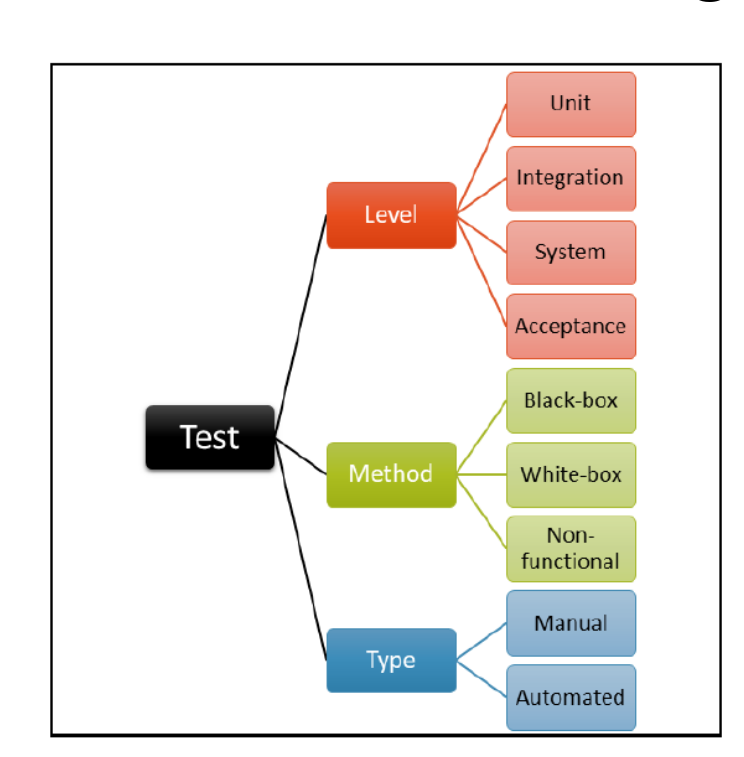
\includegraphics[width=0.50\textwidth]{img/DeAngelis/04_UnitIntegrationTesting/modello.png}
    \caption{Dimensioni ortogonali del software testing: un test può essere classificato in base al livello, al metodo e al tipo. Queste dimensioni sono indipendenti e possono combinarsi tra loro, ad esempio in un test di unità automatico white-box o in un test di sistema manuale black-box.}
    \label{fig:dimensioni-ortogonali-testing}
\end{figure}


\begin{notaprof}
Le dimensioni sono indipendenti. Non bisogna pensare che, ad esempio, i test automatici siano sempre white-box o che i test manuali siano sempre black-box. Sono classificazioni diverse che descrivono proprietà diverse del test.
\end{notaprof}

Nel metodo \textbf{black-box}, il sistema viene considerato come una scatola nera: il tester conosce input, output attesi e specifiche dell'interfaccia, ma non usa direttamente la conoscenza dell'implementazione interna.

Nel metodo \textbf{white-box}, invece, il tester conosce la struttura interna del codice e può usare questa conoscenza per progettare casi di test mirati, ad esempio per coprire specifici rami, condizioni o statement.

\section{Livelli di test e attività di V\&V}

I livelli di test possono essere rappresentati come una piramide:

\[
\text{Unit} \rightarrow \text{Integration} \rightarrow \text{System} \rightarrow \text{Acceptance}
\]

Alla base ci sono i \textbf{test di unità}, che sono numerosi, relativamente economici e
più facili da automatizzare. Salendo nella piramide, i test diventano progressivamente
più costosi, meno numerosi e spesso meno facilmente automatizzabili.
\begin{figure}[H]
    \centering
    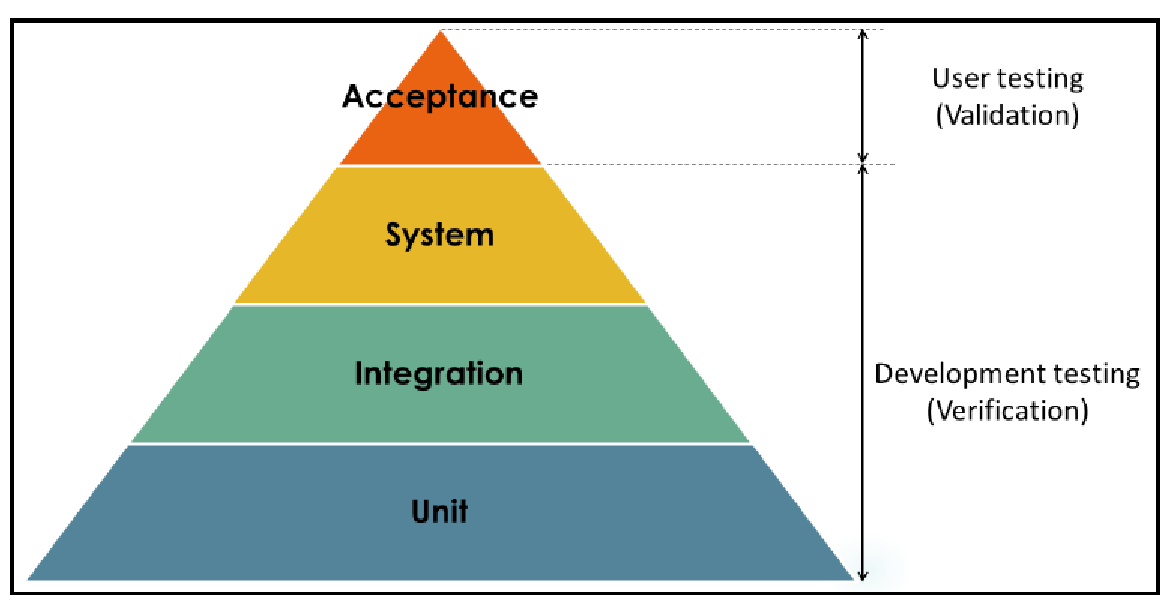
\includegraphics[width=0.65\textwidth]{img/DeAngelis/04_UnitIntegrationTesting/piramide.png}
    \caption{Piramide dei livelli di test: i test di unità, integrazione e sistema rientrano principalmente nel development testing, orientato alla verifica; i test di accettazione rientrano invece nello user testing, orientato alla validazione.}
    \label{fig:piramide-test-vv}
\end{figure}
\begin{notaslide}
La piramide dei test distingue tra \textbf{Development Testing}, associato prevalentemente alla verifica, e \textbf{User Testing}, associato prevalentemente alla validazione.
\end{notaslide}

I livelli inferiori, cioè unit, integration e system testing, rientrano tipicamente nelle attività di \textbf{verification}. Il livello di acceptance testing è invece più legato alla \textbf{validation}.

\begin{itemize}
    \item \textbf{Verification}: controlla se il prodotto è stato costruito correttamente rispetto alle specifiche. Risponde alla domanda: \emph{Are we building the product right?}
    \item \textbf{Validation}: controlla se il prodotto costruito è effettivamente quello desiderato dall'utente o dal committente. Risponde alla domanda: \emph{Are we building the right product?}
\end{itemize}

\begin{notaprof}
La verifica guarda alla conformità rispetto alle specifiche tecniche. La validazione guarda invece alla corrispondenza tra il prodotto finale e le reali aspettative dell'utente.
\end{notaprof}

\section{V-model e Continuous Testing}

Il \textbf{V-model} mette in relazione le fasi di specifica e progettazione con le corrispondenti fasi di test.

Nel ramo discendente della V si definiscono requisiti, design e codice. Nel ramo ascendente si progettano ed eseguono i test corrispondenti.

Le corrispondenze principali sono:

\begin{itemize}
    \item \textbf{Unit Design} \(\leftrightarrow\) \textbf{Unit Test};
    \item \textbf{Subsystem Design / Subsystem Requirements} \(\leftrightarrow\) \textbf{Integration Test};
    \item \textbf{System Requirements} \(\leftrightarrow\) \textbf{System Test};
    \item \textbf{Concept of Operations} \(\leftrightarrow\) \textbf{Acceptance Test}.
\end{itemize}

\begin{figure}[H]
    \centering
    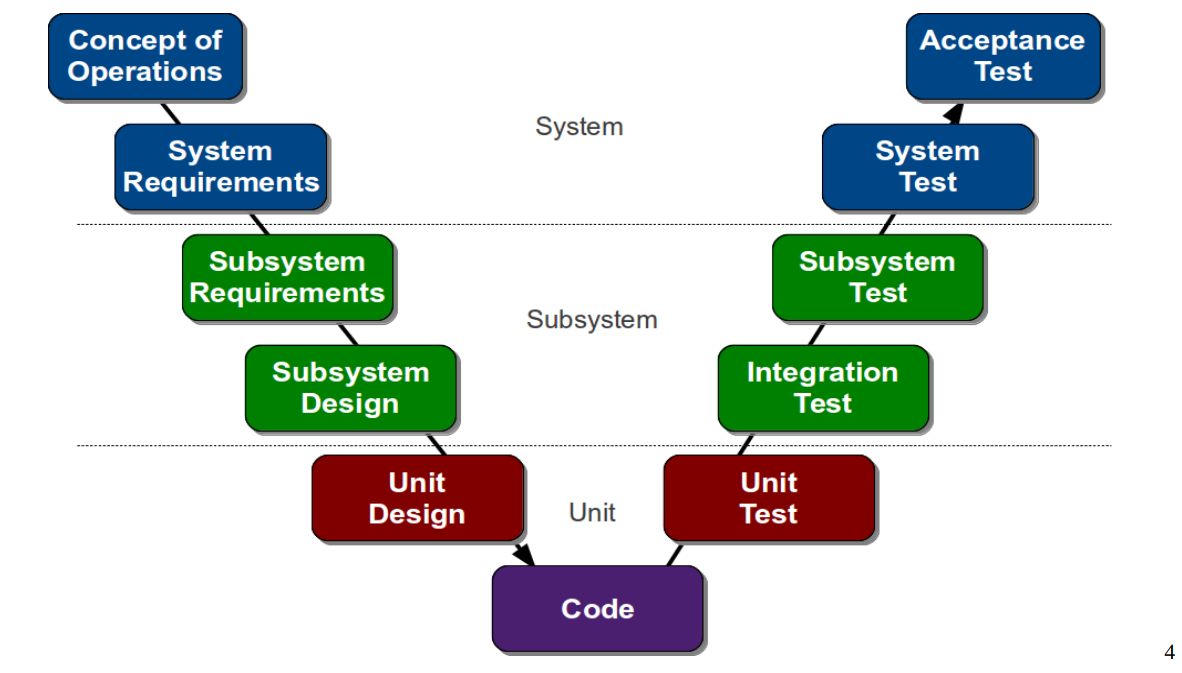
\includegraphics[width=0.7\textwidth]{img/DeAngelis/04_UnitIntegrationTesting/vmodel.png}
    \caption{V-model: relazione tra le fasi di specifica e progettazione, sul ramo discendente, e i corrispondenti livelli di test, sul ramo ascendente. Ogni livello di progettazione trova una controparte nei test: unit, integration, system e acceptance test.}
    \label{fig:vmodel-test}
\end{figure}

\begin{notaslide}
Il diagramma del V-model mostra che la progettazione dei test non dovrebbe essere vista come un'attività finale, ma come un processo collegato alle specifiche e al design delle funzionalità.
\end{notaslide}

Nel contesto del \textbf{Continuous Testing}, i casi di test vengono eseguiti automaticamente in momenti rilevanti del ciclo di sviluppo, ad esempio:

\begin{figure}[H]
    \centering
    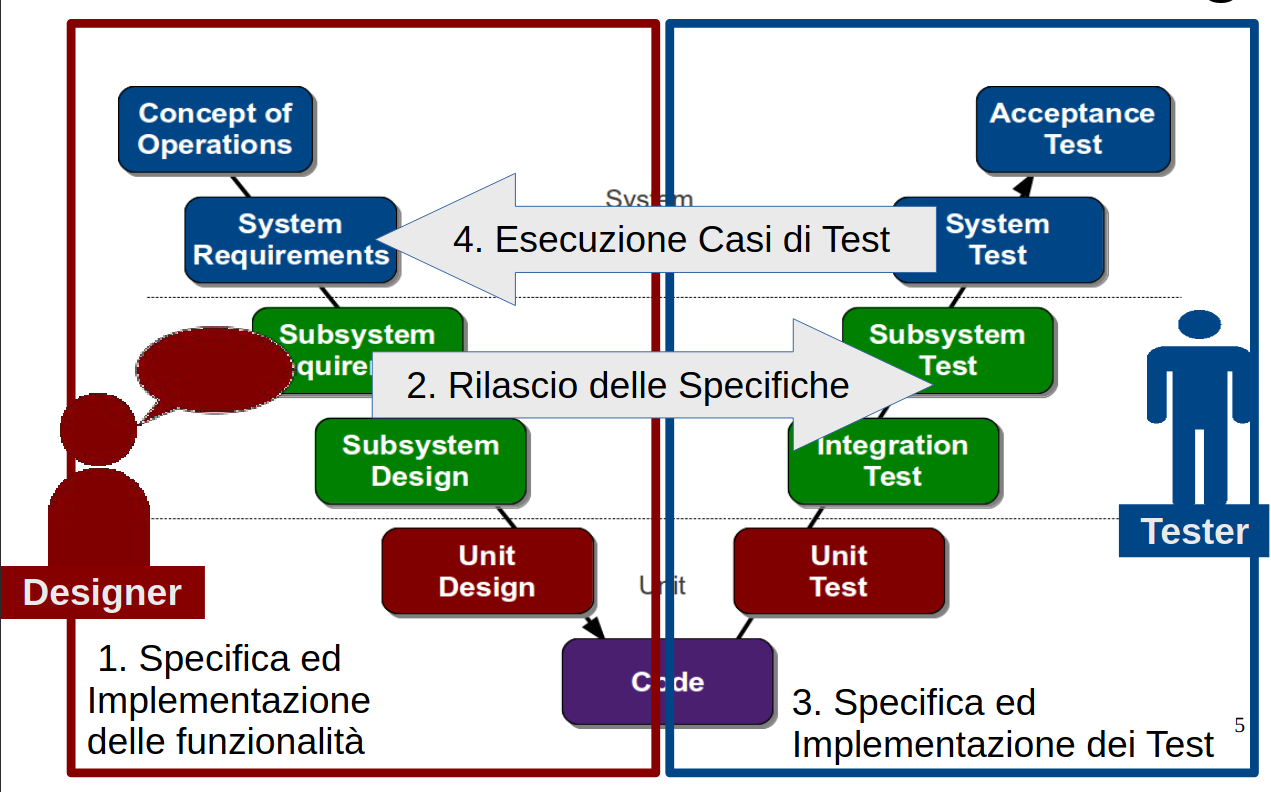
\includegraphics[width=0.9\textwidth]{img/DeAngelis/04_UnitIntegrationTesting/ct.png}
    \caption{V-model nel contesto del Continuous Testing: il designer specifica e implementa le funzionalità, rilascia le specifiche al tester, il tester progetta e implementa i casi di test, che vengono poi eseguiti automaticamente durante il ciclo di sviluppo.}
    \label{fig:vmodel-continuous-testing}
\end{figure}

\begin{itemize}
    \item a ogni proposta di modifica, come commit o Pull Request;
    \item al rilascio di una nuova funzionalità;
    \item al rilascio di una nuova versione.
\end{itemize}

\begin{notaprof}
Il processo di testing vive in parallelo allo sviluppo. Il designer produce specifiche e funzionalità; il tester usa tali informazioni per progettare casi di test. In un contesto continuo, i test vengono rieseguiti automaticamente ogni volta che il sistema cambia.
\end{notaprof}

\section{Test di unità}

I \textbf{test di unità} hanno l'obiettivo di rivelare malfunzionamenti relativi a un singolo modulo o a una singola unità funzionale del \textbf{System Under Test}.

Lo scopo è acquisire confidenza che ogni unità, se eseguita in isolamento, si comporti come atteso.

Una unità può essere, a seconda del contesto:

\begin{itemize}
    \item una funzione;
    \item un metodo;
    \item una classe;
    \item un modulo;
    \item un package;
    \item una piccola unità funzionale del sistema.
\end{itemize}

Generalmente i test di unità sono definiti direttamente dagli sviluppatori delle unità del SUT.

Possono essere progettati secondo due prospettive:

\begin{itemize}
    \item \textbf{White-box}: usando come riferimento l'implementazione realizzata;
    \item \textbf{Black-box}: usando come riferimento la funzionalità astratta da realizzare, il modello comportamentale o gli esempi descritti dalle specifiche.
\end{itemize}

\begin{notaslide}
Le slide richiamano anche il \textbf{Test Driven Development} (TDD), in cui i test possono essere sviluppati prima della scrittura del codice.
\end{notaslide}

L'adeguatezza di una suite di unit test può essere valutata in funzione di:

\begin{itemize}
    \item numero di funzionalità controllate;
    \item numero di requisiti controllati;
    \item numero di aspetti rilevabili dalle specifiche;
    \item metriche di copertura del codice sorgente.
\end{itemize}

\begin{notaesame}
Il test di unità verifica che una singola unità funzioni correttamente in isolamento. Non è pensato per verificare la correttezza dell'interazione tra più moduli: quello è compito del test di integrazione.
\end{notaesame}

\section{JUnit: obiettivi e filosofia}

\textbf{JUnit} è un framework che supporta l'implementazione di unit test in ambienti Java.

I principali obiettivi di JUnit sono:

\begin{itemize}
    \item supportare la definizione di casi di test utili;
    \item supportare la definizione di casi di test ripetibili nel tempo;
    \item ridurre i costi di scrittura dei casi di test tramite pratiche orientate al riuso del codice.
\end{itemize}

JUnit non è un linguaggio separato, ma un framework Java basato su classi, metodi, annotazioni e asserzioni.

\begin{notaesame}
JUnit è uno strumento per \textbf{implementare} ed \textbf{eseguire} casi di test e test suite. Non decide quale strategia di test usare, quali test siano più significativi o quali valori di input selezionare.
\end{notaesame}

Questo significa che JUnit fornisce l'infrastruttura esecutiva, ma la qualità del test dipende comunque dal lavoro del progettista dei test.

\section{Esempi JUnit: test parametrizzati}

I \textbf{test parametrizzati} permettono di eseguire lo stesso test più volte con coppie o tuple diverse di input e output attesi.

In JUnit 4, una classe di test parametrizzata può usare:

\begin{verbatim}
@RunWith(Parameterized.class)
\end{verbatim}

Questa annotazione indica a JUnit che la classe deve essere eseguita tramite il runner parametrizzato.

La struttura tipica prevede:

\begin{itemize}
    \item attributi privati per memorizzare i parametri del test;
    \item un metodo annotato con \texttt{@Parameters};
    \item un costruttore con tanti argomenti quanti sono i parametri;
    \item uno o più metodi annotati con \texttt{@Test}.
\end{itemize}

Il metodo annotato con \texttt{@Parameters} deve essere statico e restituire una \texttt{Collection} contenente le tuple di valori da usare nei test.

\begin{notaprof}
Il metodo \texttt{@Parameters} deve essere statico perché JUnit deve recuperare i parametri prima di creare le istanze della classe di test.
\end{notaprof}

Un esempio schematico è:

\begin{verbatim}
@RunWith(Parameterized.class)
public class ParameterizedTest {

    private double expected;
    private double valueOne;
    private double valueTwo;

    @Parameters
    public static Collection<Integer[]> getTestParameters() {
        return Arrays.asList(new Integer[][] {
            {2, 1, 1},
            {3, 2, 1},
            {4, 3, 1}
        });
    }

    public ParameterizedTest(double expected,
                             double valueOne,
                             double valueTwo) {
        this.expected = expected;
        this.valueOne = valueOne;
        this.valueTwo = valueTwo;
    }

    @Test
    public void sum() {
        Calculator calc = new Calculator();
        assertEquals(expected, calc.add(valueOne, valueTwo), 0);
    }
}
\end{verbatim}

\begin{notaslide}
Nell'esempio delle slide, il test parametrizzato usa il runner JUnit, parametri come attributi privati, un metodo di configurazione che restituisce una \texttt{java.util.Collection} e un costruttore con tanti argomenti quanti sono i parametri.
\end{notaslide}

\section{Pre-testing e post-testing globale}

JUnit fornisce annotazioni per definire azioni da eseguire prima o dopo i test.

Le annotazioni globali sono:

\begin{itemize}
    \item \texttt{@BeforeClass}: metodo eseguito una sola volta prima di tutti i test della classe;
    \item \texttt{@AfterClass}: metodo eseguito una sola volta dopo tutti i test della classe.
\end{itemize}

Questi metodi vengono usati per operazioni di setup o teardown globale, come inizializzare risorse condivise o chiudere risorse alla fine dell'intera suite.

\begin{notaslide}
Le slide precisano che non è specificato un ordine di esecuzione tra più metodi annotati con \texttt{@BeforeClass}, né tra più metodi annotati con \texttt{@AfterClass} ovvero è \textbf{NON deterministico}.
\end{notaslide}

Le annotazioni locali sono invece:

\begin{itemize}
    \item \texttt{@Before}: metodo eseguito prima di ogni singolo test;
    \item \texttt{@After}: metodo eseguito dopo ogni singolo test.
\end{itemize}

\begin{notaprof}
\texttt{@BeforeClass} e \texttt{@AfterClass} lavorano una volta per tutta la classe. \texttt{@Before} e \texttt{@After} lavorano invece prima e dopo ogni singolo test, garantendo maggiore isolamento tra i casi di test.
\end{notaprof}

Il flusso logico può essere rappresentato così:

\[
\texttt{@BeforeClass}
\rightarrow
(\texttt{@Before} \rightarrow \texttt{@Test} \rightarrow \texttt{@After})
\rightarrow
\texttt{@AfterClass}
\]

\section{Designer dei test e programmatore dei test}

Nel processo di testing è importante distinguere tra due responsabilità logiche:

\begin{itemize}
    \item \textbf{designer dei casi di test};
    \item \textbf{programmatore dei casi di test}.
\end{itemize}

Il \textbf{designer} identifica dettagliatamente i valori attesi da un test. Può farlo usando:

\begin{itemize}
    \item valori puntuali;
    \item specifiche;
    \item un oracolo;
    \item una funzione di predizione;
    \item un sistema esterno equivalente.
\end{itemize}

Il \textbf{programmatore} implementa invece le scelte progettuali attraverso istruzioni di verifica e controllo, ad esempio usando \texttt{assertEquals}, \texttt{assertTrue} o altre asserzioni.

\begin{notaesame}
Un test senza valori attesi e senza assert significative è incompleto. Chiamare un metodo senza verificare il risultato non basta: bisogna stabilire un oracle e codificarlo nel test.
\end{notaesame}

\begin{notaprof}
Nello unit testing, designer e programmatore dei test spesso coincidono con lo sviluppatore. Tuttavia, concettualmente sono ruoli diversi: il designer decide cosa testare e quale risultato aspettarsi; il programmatore decide come codificare la verifica.
\end{notaprof}

\section{Test di integrazione}

I \textbf{test di integrazione} hanno l'obiettivo di far emergere malfunzionamenti derivanti dall'interazione tra due o più moduli o componenti del SUT.

Questi test servono ad acquisire confidenza sul fatto che:

\begin{itemize}
    \item esistano le dovute interconnessioni tra moduli o componenti;
    \item le interazioni rispettino i contratti funzionali;
    \item i protocolli e le specifiche di interazione siano rispettati.
\end{itemize}

\begin{notaprof}
Un esempio classico è un sensore di temperatura progettato in Europa che invia gradi Celsius a una centralina sviluppata negli Stati Uniti che si aspetta gradi Fahrenheit. I due moduli possono funzionare perfettamente se testati isolatamente, ma fallire quando vengono integrati.
\end{notaprof}

L'assunzione alla base dell'integration testing è che ogni modulo o unità funzionale, preso in isolamento, si comporti già correttamente. In altre parole, si assumono superati i test di unità.

I test di integrazione possono essere scritti da:

\begin{itemize}
    \item sviluppatori;
    \item integratori;
    \item tester.
\end{itemize}

La scelta dipende dagli scenari di integrazione considerati.

I test possono essere progettati:

\begin{itemize}
    \item in modalità \textbf{white-box}, assumendo disponibilità del codice dei moduli;
    \item in modalità \textbf{black-box}, assumendo disponibilità solo delle specifiche di interazione;
    \item in modalità mista, che nella pratica è molto frequente.
\end{itemize}

\begin{notaprof}
Nella pratica spesso si conosce bene il proprio modulo, ma si trattano le dipendenze esterne come scatole nere. Per questo l'approccio reale è spesso misto.
\end{notaprof}

\begin{notaesame}
Il test di integrazione non serve a ritestare la logica interna del singolo modulo. Serve a verificare che più moduli comunichino correttamente e rispettino i contratti stabiliti.
\end{notaesame}

\section{Stub, mock e test driver}

Nei test incrementali si considerano solo parti del SUT. Di conseguenza, alcune dipendenze potrebbero:

\begin{itemize}
    \item non essere ancora disponibili;
    \item essere troppo costose da usare;
    \item essere lente o instabili;
    \item non dover essere realmente invocate nello specifico test.
\end{itemize}

Per questo motivo si usano stub, mock e test driver.

\subsection{Stub e mock}

Uno \textbf{stub} è un elemento software definito in fase di test. Può essere una classe, un modulo, una unità o un componente fittizio.

Le sue caratteristiche sono:

\begin{itemize}
    \item non è soggetto a test;
    \item fa parte dell'ambiente di test;
    \item simula il comportamento di una unità mancante;
    \item spesso restituisce comportamenti banali, costanti o controllati.
\end{itemize}

Il termine \textbf{mock} viene spesso usato per indicare un oggetto finto che simula una dipendenza e consente anche di verificare le interazioni avvenute.

\begin{notaprof}
Se si vuole testare un componente che dipende da un database, può essere utile usare un mock del database. In questo modo si verifica la logica del componente senza dipendere realmente dal database.
\end{notaprof}

\subsection{Test driver}

Il \textbf{test driver} è l'esecutore del test. Invoca i moduli coinvolti e spesso codifica parte della logica di integrazione che si vuole ottenere dai moduli composti.

Un driver semplice si limita a chiamare il codice da testare. Un driver più avanzato può occuparsi anche di:

\begin{itemize}
    \item configurazione dell'ambiente di test;
    \item coordinamento delle risorse;
    \item clean-up dopo l'esecuzione;
    \item gestione del contesto necessario al test.
\end{itemize}

\begin{notaesame}
Stub e mock simulano dipendenze richieste dal SUT. Il test driver, invece, guida l'esecuzione del test e coordina l'interazione tra i componenti.
\end{notaesame}
